\documentclass[12pt]{article} 

%?? paths
\newcommand{\CiteMathPackage}{../../math} 
\newcommand{\CiteReference}{../reference.bib}

%?? packages 
\usepackage{setspace,geometry,fancyvrb,rotating} 
\usepackage{marginnote,datetime,enumitem} 
\usepackage{titlesec,indentfirst} 
\usepackage{amsmath,amsfonts,amssymb,amsthm,mathtools} 
\usepackage{threeparttable,booktabs,adjustbox} 
\usepackage{graphicx,epstopdf,float,soul,subfig} 
\usepackage[toc,page]{appendix} 
\usdate

%?? page setup 
\geometry{scale=0.8} 
\titleformat{\paragraph}[runin]{\itshape}{}{}{}[.] 
\titlelabel{\thetitle.\;} 
\setlength{\parindent}{10pt} 
\setlength{\parskip}{10pt} 
\usepackage{Alegreya} 
\usepackage[T1]{fontenc}
% \usepackage{fourier} % Favorite Font

%?? bibliography 
\usepackage{natbib,fancybox,url,xcolor} 
\definecolor{MyBlue}{rgb}{0,0.2,0.6} 
\definecolor{MyRed}{HTML}{D2042D}
\definecolor{MyGreen}{rgb}{0,0.4,0} 
\definecolor{MyPink}{HTML}{E50379} 
\definecolor{MyOrange}{HTML}{CC5500} 
\definecolor{MyPurple}{HTML}{BF40BF}
\newcommand{\highlightR}[1]{{\emph{\color{MyRed}{#1}}}} 
\newcommand{\highlightB}[1]{{\emph{\color{MyBlue}{#1}}}} 
\newcommand{\highlightP}[1]{{\emph{\color{MyPink}{#1}}}} 
\newcommand{\highlightO}[1]{{\emph{\color{MyOrange}{#1}}}}
\newcommand{\highlightPP}[1]{{\emph{\color{MyPurple}{#1}}}}
\usepackage[bookmarks=true,bookmarksnumbered=true,colorlinks=true,linkcolor=MyGreen,citecolor=MyGreen,filecolor=MyBlue,urlcolor=MyGreen]{hyperref} 
\bibliographystyle{econ}

%?? math and theorem environment 
\theoremstyle{definition} 
\newtheorem{assumption}{Assumption} 
\newtheorem{definition}{Definition} 
\newtheorem{theorem}{Theorem} 
\newtheorem{proposition}{Proposition} 
\newtheorem{lemma}{Lemma} 
\newtheorem{example}{Example} 
\newtheorem{result}{Result} 
\newtheorem{corollary}[theorem]{Corollary} 
\usepackage{mathtools} 
\usepackage{\CiteMathPackage}

\begin{document} 

%??%??%??%??%??%??%??%??%??%??%??%??%??%??%??%??%??%??%??%??%??%?? 
%?? title 
%??%??%??%??%??%??%??%??%??%??%??%??%??%??%??%??%??%??%??%??%??%??

\title{\bf Occupation Growth, Skill Prices, and Wage Inequality, Journal of Labor Economics, 2024} 
\author{Wenzhi Wang \thanks{This note is written in my pre-doc period at the University of Chicago Booth School of Business.} } 
\date{\today} 
\maketitle 

\citet{bohmOccupationGrowthSkill2024}

\section{Introduction}

During the past decades, occupational employment has changed profoundly across Europe and the United States. A burgeoning literature has established fundamental shifts in labor demand as the most important cause of these changes. Yet it remains puzzling that these demand shifts fail to be clearly reflected in occupational wages or wage inequality. First, occupational employment growth has been decoupled from occupational wage growth. Second, a number of studies suggest that changes in occupation-specific labor demand contributed little to the increase in wage inequality in recent decades. 

Making use of individual-level longitudinal information on wages and occupations from German administrative data, we document three important facts. First, individual workers' wage growth is substantially faster within expanding occupations. During our study period (1985-2010), annual individual wage growth is $1$ percentage point higher on average in occupations that double in size compared with those whose size is constant. Second, workers who enter an occupation earn $21\%$ less than incumbents on average. Similarly, average wages of workers leaving occupations are $16\%$ lower than those of stayers. Third, both of these effects are increasing in net occupation growth. For a doubling in occupation size, the wage gaps between entrants versus incumbents and between leavers versus stayers widen by $6$ and $3$ percentage points, respectively. The raw data thus reveal that net growth of an occupation will attenuate average wages within occupations where selection operates in both directions. This explains why wage and employment growth across occupations are uncorrelated in our data. 

To interpret these facts, we set up a parsimonious model of occupation choice. Workers have multidimensional occupation-specific skills that evolve heterogeneously across occupations and over the career. \highlightR{The central distinction we make is between skill prices -- wages paid per constant unit of skill -- and average occupational wages.} \highlightP{While skill prices are directly affected by shifts in demand, selection may dampen, neutralize, or even overturn their effects on average wages.} Less skilled individuals enter growing occupations, which depress these occupations' average wages. Shrinking occupations also retain the most skilled parts of their workforce, lifting their average wages. Such selection effects imply that between-occupation inequality will underestimate the impact of shifting occupational demand on wage inequality.

We estimate the model using the longitudinal information in our data. Our analysis uncovers three main findings. \highlightP{First, there is a clear positive relation between skill price and employment growth at the level of detailed occupations.} This indicates that demand shifts were the dominant drivers of both occupational employment and skill-constant wages over the past decades. Characterizing occupations by their task intensities, we find that the patterns are in line with routine-based technical change as one of the important drivers of occupational demand. More generally, the patterns are consistent with polarization, since employment and skill prices of broad occupation groups with high as well as low wages rose compared with those of midwage occupation groups. 

Since employment growth is uncorrelated with average wage growth and is positively correlated with skill price growth, skills must deteriorate in growing occupations and increase in shrinking occupations. \highlightP{Our second main finding is that lower-earning workers' net entry into growing occupations and their net exit out of shrinking occupations fully account for the negative relationship between skill changes and employment growth.} We term this the ``employment growth selection effect,'' or simply growth selection. Quantitatively, a doubling of an occupation's workforce translates into a decrease in its average skills by $12\%$. Viewed through the lens of our model, growth selection stems from both entrants and leavers possessing lower average skills than stayers in any occupation. We exploit the longitudinal dimension of the data to document the nature of growth selection. One component is that growing occupations draw in and shed younger workers who are equally skilled as inframarginal workers but who have had less time to accumulate skills because of their age. We distinguish this age selection from Roy selection, which refers to differences in skills conditional on experience. Because of the fundamental selection problem, we focus on the current spell in a particular occupation. Aggregating across occupation groups, we find that $42\%$ of employment growth selection can be attributed to age selection.

\highlightP{Our third findings is that changes in occupational skill prices have driven much of the increase in wage inequality over the past decades.} Inequality between occupations would have been $70\%$ higher at the end of our sample if growth selection had not counteracted the changing skill prices. We break down the quantiles of the wage distribution using our estimates of skill prices and skills along with workers' occupational histories. Our model tracks the wage distribution well. Demographic composition and faster skill accumulation at the median can account for $70\%$ of the rise in the fiftieth to fifteenth percentile wage difference. Controlling for other factors, skill prices alone explain $60\%$ of the increase in the eighty-fifth to fiftieth percentile difference.

\section{Data, Literature, and Stylized Facts}

To work with a homogenous sample throughout, we restrict the main sample to German men aged 25-54 years who are working full tim (excluding apprentices) in West Germany. We transform the spell structure into a yearly panel by using the longest spell in any given year, adjusting wages appropriately for spells that do not last the entire year. Because of a cap on social security contributions, $12\%$ of wages are right censored at this ceiling; we follow the imputation procedures in past papers. We inflate all wages to 2010 prices using the German consumer price index.

A key strength of the SIAB data is that it provides high-quality longitudinal information on workers' occupations. Until 2010, the SIAB scientific use file contains a consistent set of 120 occupations; we cannot use subsequent years because the classification changes drastically thereafter. Most of our analyses will be based on the raw 120 occupations. To ease interpretation, we also aggregate them into broader groups. These comprise managers, professionals, and technicians (Mgr-Prof-Tech); sales and office workers (Sales-Office); production workers, operators, and craftsmen (Prod-Op-Crafts); and workers in services and care occupations (Srvc-Care). See table A.1 for the mapping of detailed occupations into these groups.

\subsection{Wage Inequality and Changes in Occupational Employment}

\highlightP{Two of the most important trends in developed countries' labor markets over the past decades have been a strong increase in wage inequality and a substantial reallocation of employment across occupations broadly characterized by polarization.} Germany is no exception to either phenomenon. Figure \ref{bohmOccupationGrowthSkill2024_fig1} reproduces both trends in our dataset.

\begin{figure}[H]
    \noindent\caption{Evolution of wage inequality and occupational employment}
    \begin{center}
        \resizebox{1\textwidth}{!}{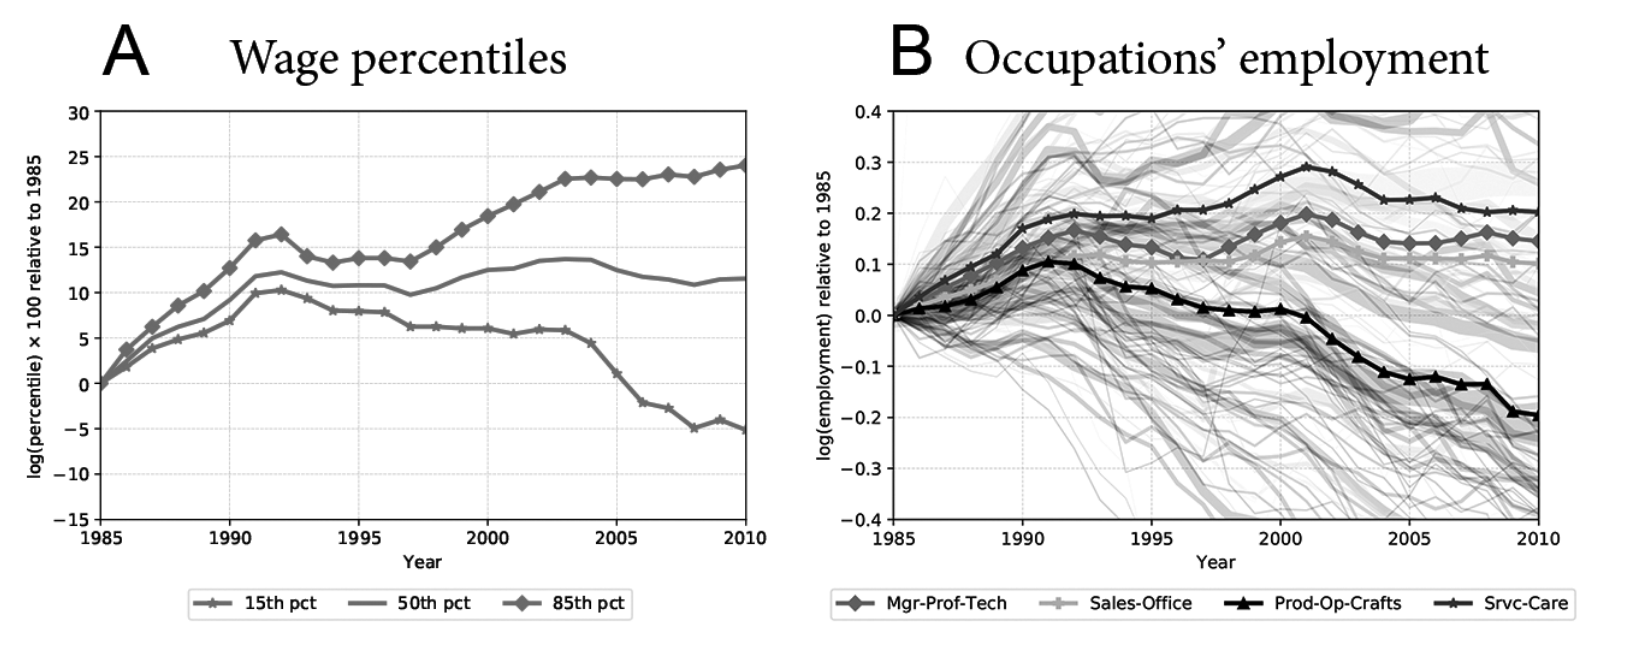
\includegraphics{bohmOccupationGrowthSkill2024_fig1.png}}
        \label{bohmOccupationGrowthSkill2024_fig1}
    \end{center}

    {\footnotesize Notes. The vertical axis in A shows the fifteenth, fiftieth, and eighty-fifth log wage percentile over time relative to 1985. The vertical axis in B shows the log change in the number of employed workers within an occupation over time. Shaded lines in the background represent the 120 detailed occupations in the SIAB scientific use file. The four groups show an aggregation of these detailed occupations, as described in table A.1. The thickness of a shaded background line corresponds to the number of employed workers in an occupation averaged across years 1985 until 2010. A color version of this figure is available online.}
\end{figure}

Figure \ref{bohmOccupationGrowthSkill2024_fig1}A shows the trends of wage percentiles over the 1985-2010 period normalized to zero in 1985. Inequality increased strongly and steadily both in the upper half, measured by the difference between the eighty-fifth and fiftieth percentile of log wages, and in the lower half (50 - 15 difference). Figure \ref{bohmOccupationGrowthSkill2024_fig1}B plots the trends in the logs of the detailed 120 occupations' employment (shaded lines) and the four aggregated groups (bold lines with markers). Employment in Prod-Op-Crafts occupations declined by more than $20$ log points from a baseline share of more than $60\%$, whereas the employment share of the other occupation groups increased. This trend has been termed ``job'' or ``employment polarization'' because Prod-Op-Crafts workers tend to be located in the middle of the occupational wage distribution. Part of the declining employment in middle-paying occupations appears to be due to changes in technology (affecting codifiable routine-type jobs) as well as international trade and offshoring (affecting manufacturing-type jobs).

One may expect to see such shifts of the demand for different types of occupations directly in the wage distribution, not least because the wage and employment trends occurred largely in parallel. There exists, however, surprisingly little quantitative evidence on the role of occupational change for the evolution of wage inequality: holding occupations' wages fixed at their initial levels and reweighting them with employment in subsequent decades, Goos and Manning (2007) show that composition effects due to employment polarization can account for a substantial part of changing wage inequality in the United Kindom. Autor (2019) finds that in the United States, a similar exercise explains only small shares of the income differentials across five education groups. For the German case, Dustmann, Ludsteck, and Schönberg (2009) conclude that the rise of lower-half inequality was unlikely to stem from changes in demand. Card, Heining, and Kline (2013) run a set of Mincer regressions and incrementally add occupational identifiers, finding that the role of the latter for rising wage inequality is rather small.

\begin{figure}[H]
    \noindent\caption{Correlation of changes in employment, average wages, and wage growth}
    \begin{center}
        \resizebox{1\textwidth}{!}{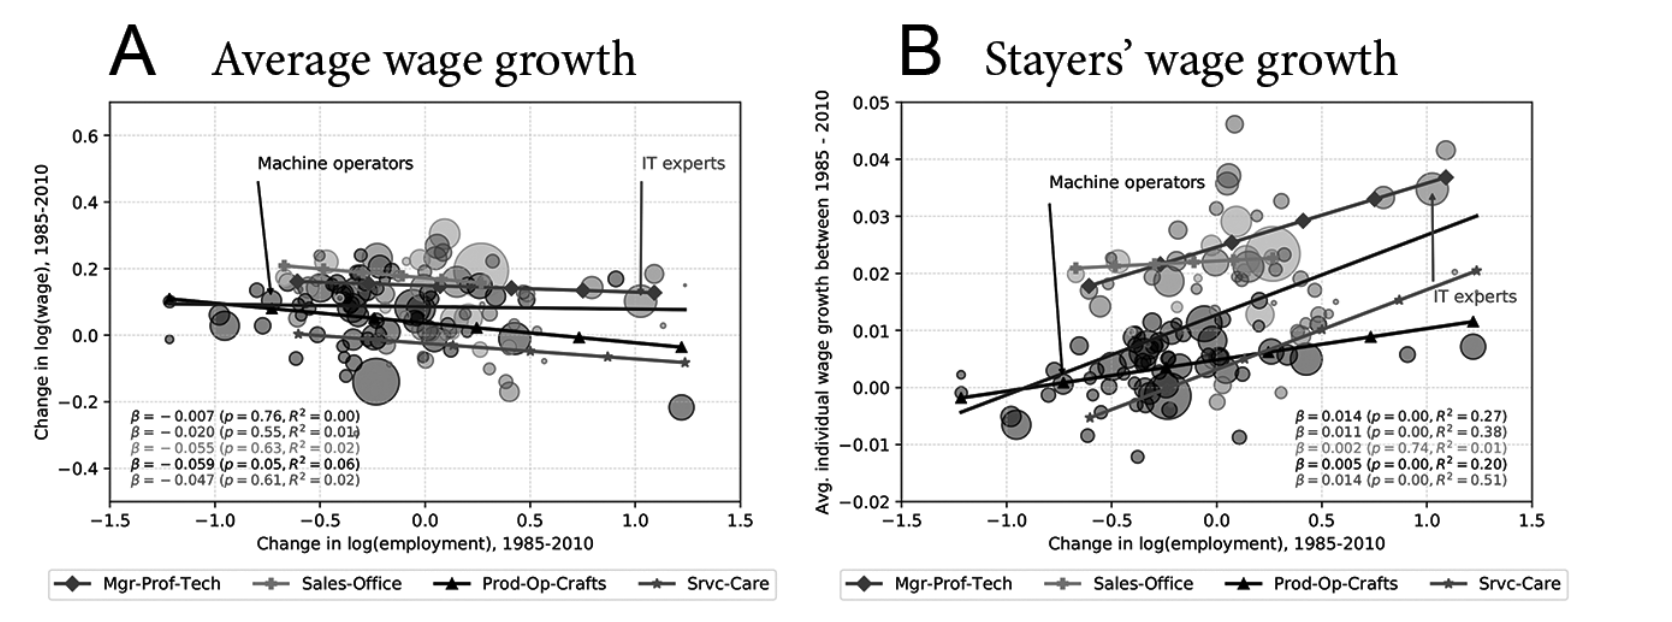
\includegraphics{bohmOccupationGrowthSkill2024_fig2.png}}
        \label{bohmOccupationGrowthSkill2024_fig2}
    \end{center}
    \vspace{-20pt}
    {\footnotesize Notes. The vertical axis in A shows the change in average wages between 1985 and 2010. The vertical axis in B depicts individual wage growth averaged across years 1985 until 2010. The horizontal axis in both panels shows the change of the log number of employed workers within an occupation between 1985 and 2010. One bubble represents one of the 120 detailed occupations in the SIAB scientific use file. The four groups show an aggregation of these detailed occupations, as described in table A.1. Bubble size corresponds to the number of employed workers in an occupation averaged across years 1985 until 2010. Regression lines across all occupations (black) and within the four broad groups (symbols) are weighted by the number of employed workers. A color version of this figure is available online.}
\end{figure}

Figure \ref{bohmOccupationGrowthSkill2024_fig2}A hints at why these analyses tend to have limited explanatory power, plotting changes in employment against changes in average wages over the 1985-2010 period for each occupation. Variation along the horizontal axis shows that employment changes are very substantial. Many occupations grew or shrank by more than $50$ log points. Yet movements of average wages are surprisingly small. \highlightP{Thus, between-occupation decompositions -- such as wage regressions with occupation dummies or reweighting strategies -- may attribute little of the trends of in wage inequality to factors like changing skill prices and employment structure and much of its increase to unexplained within-occupation inequality.} In fact, the regression line shows that employment and wage changes are uncorrelated. To pick the two highlighted examples, information technology (IT) experts' employment rose by $102$ log points, or $178\%$. Their average wages grew by $10\%$, just above the overall average. Machine operators—a prototypical occupation to be hit by RBTC—shrank by $73$ log points, or $51\%$. Yet average wages grew by the same amount as those of IT experts.

Within the broader groups, the noncorrelation between wage and employment growth even turns negative for the lower-earning Prod-OpCrafts and Srvc-Care occupations. This is consistent with the regressions reported by Dustmann, Ludsteck, and Schönberg (2009, sec. IV.D). They conclude that demand shifts were unlikely to have driven lower-end inequality. Finding little or negative correlation between occupational wage and employment growth is not confined to Germany. Hsieh et al. (2019) and Roys and Taber (2019) document very small correlations between the growth rates of occupational employment and wages in the United States. Employment in low-skill occupations increased in the United Kingdom and Canada, while at the same time wages dropped compared with routine occupations (Goos and Manning 2007; Green and Sand 2015). 

\highlightP{Next to the role that occupations have to play for wage inequality, this begets the more fundamental question of whether, on aggregate, shifts in demand versus supply of labor to different occupations were the dominant factor for the changes of the employment structure.} We will find that while the latter may have a role to play, the data strongly suggest that demand changes along the lines of routine-biased technological or international trade are important.

\subsection{Individual-Level Wage Growth and Selection}

As a first pass, figure \ref{bohmOccupationGrowthSkill2024_fig2}B shows that there is a strong positive correlation between employment and individual-level wage growth. The horizontal axis is the same as in figure \ref{bohmOccupationGrowthSkill2024_fig2}A, whereas the vertical axis plots the average annual wage growth of workers who stayed in their occupation for any two consecutive years. Wage growth rates within occupations clearly line up with their employment growth. We will control for other important factors, such as occupation- and age-specific returns to experience, below. But the juxtaposition of figure \ref{bohmOccupationGrowthSkill2024_fig2}A and \ref{bohmOccupationGrowthSkill2024_fig2}B already suggests that the key reason for the differences will be selection into occupations. \highlightP{Put differently, demand shifts will indeed be driving the changes of employment and prices paid for skilled labor across occupations. Negative selection of entrants into growing occupations obscures this relation when looking at average occupation-specific wages.} The underlying occupational prices would be spreading out more than the average occupational wages, which are captured in the above-discussed decomposition analyses.

Data limitations have prevented a more thorough analysis of such selection effects. In particular, the main sources in the United States are repeated cross sections (Current Population Survey [CPS], US Census) or longitudinal data too small in size for investigating individual-level dynamics across detailed occupations (Panel Study of Income Dynamics [PSID], National Longitudinal Survey of Youth). The SIAB data allow us to track occupational biographies over the entire career.

\begin{figure}[H]
    \noindent\caption{Selection into and out of occupations}
    \begin{center}
        \resizebox{1\textwidth}{!}{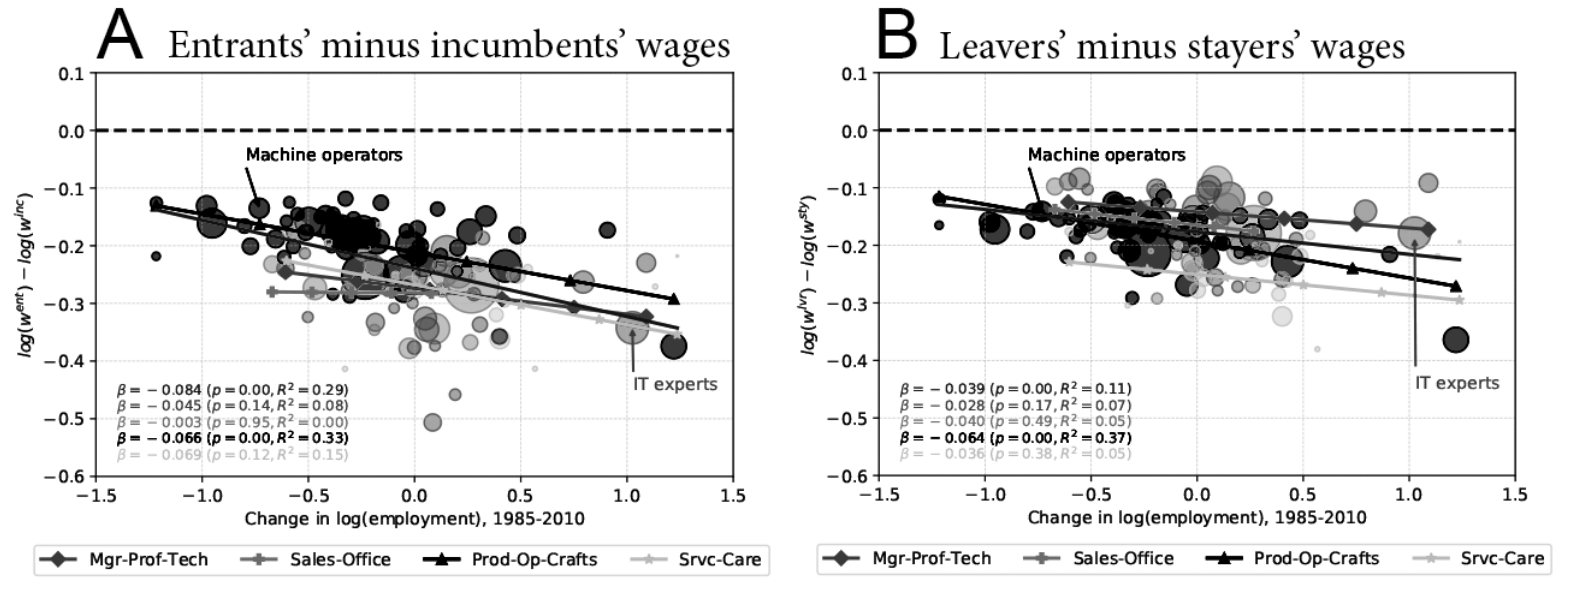
\includegraphics{bohmOccupationGrowthSkill2024_fig3.png}}
        \label{bohmOccupationGrowthSkill2024_fig3}
    \end{center}
    \vspace{-20pt}
    {\footnotesize Notes. The vertical axis in A shows the average wage of an entrant to an occupation relative to the average wage of incumbents. The average wage is taken across years 1985 until 2010. The vertical axis in B shows the average wage of a worker leaving an occupation next period relative to the average wage of stayers. The average is taken across years 1985 until 2009 to avoid all workers being leavers at the sample end. The horizontal axis in both panels shows the change in the log number of employed workers within an occupation between 1985 and 2010. One bubble represents one of the 120 detailed occupations in the SIAB scientific use file. The four groups show an aggregation of these detailed occupations, as described in table A.1. Bubble size corresponds to the number of employed workers in an occupation averaged across years 1985 until 2010. Regression lines across all occupations (black) and within the four broad groups (symbols) are weighted by the number of employed workers. A color version of this figure is available online.}
\end{figure}

The vertical axis of figure \ref{bohmOccupationGrowthSkill2024_fig3}A shows the difference between entrants and incumbents. An occupational entrant is someone newly observed in the occupation in the current period. He could be joining the labor force for the first time, switch from a different occupation, or enter from unemployment or outside the labor force. The wage difference between this group and incumbents is strongly negative.

In principle, the patterns in figure \ref{bohmOccupationGrowthSkill2024_fig3}A could be generated if occupation choice happened only at labor market entry in combination with substantial returns to experience. If this was the sole effect, however, we would expect that the wages of workers leaving their occupations would be higher than the wages of those who stay on. Put differently, in such a scenario individuals dropping out of our sample after age 54 should dominate the difference between leavers and stayers. Figure \ref{bohmOccupationGrowthSkill2024_fig3}B and \ref{bohmOccupationGrowthSkill2024_tab1} show that the opposite is the case. As for entrants, marginal workers have substantially lower wages than those who stay on. This difference is $17.5$ log points on average and increases by $3.9$ log points per $100$ log points higher employment growth. Put differently, only the lowest-skilled workers leave fast-growing occupations. This suggests that the wage gap is not just due to entrants being at an earlier stage of their career than incumbents.

The second specification in \ref{bohmOccupationGrowthSkill2024_tab1} investigates how much of the wage gaps can be explained with standard observable skill proxies. \highlightPP{We first run Mincer regressions of individual workers' wages on full interactions of dummies for calendar year, education in three categories, and years of age. We use the residuals to compute the average wage gaps for entrants/leavers and their slopes with respect to occupation growth as before.}
\setcounter{figure}{0}
\renewcommand{\thefigure}{Table \arabic{figure}}
\begin{figure}[H]
    \noindent\caption{Selection Into and Out of Occupations: Regression Results}
    \begin{center}
        \resizebox{0.7\textwidth}{!}{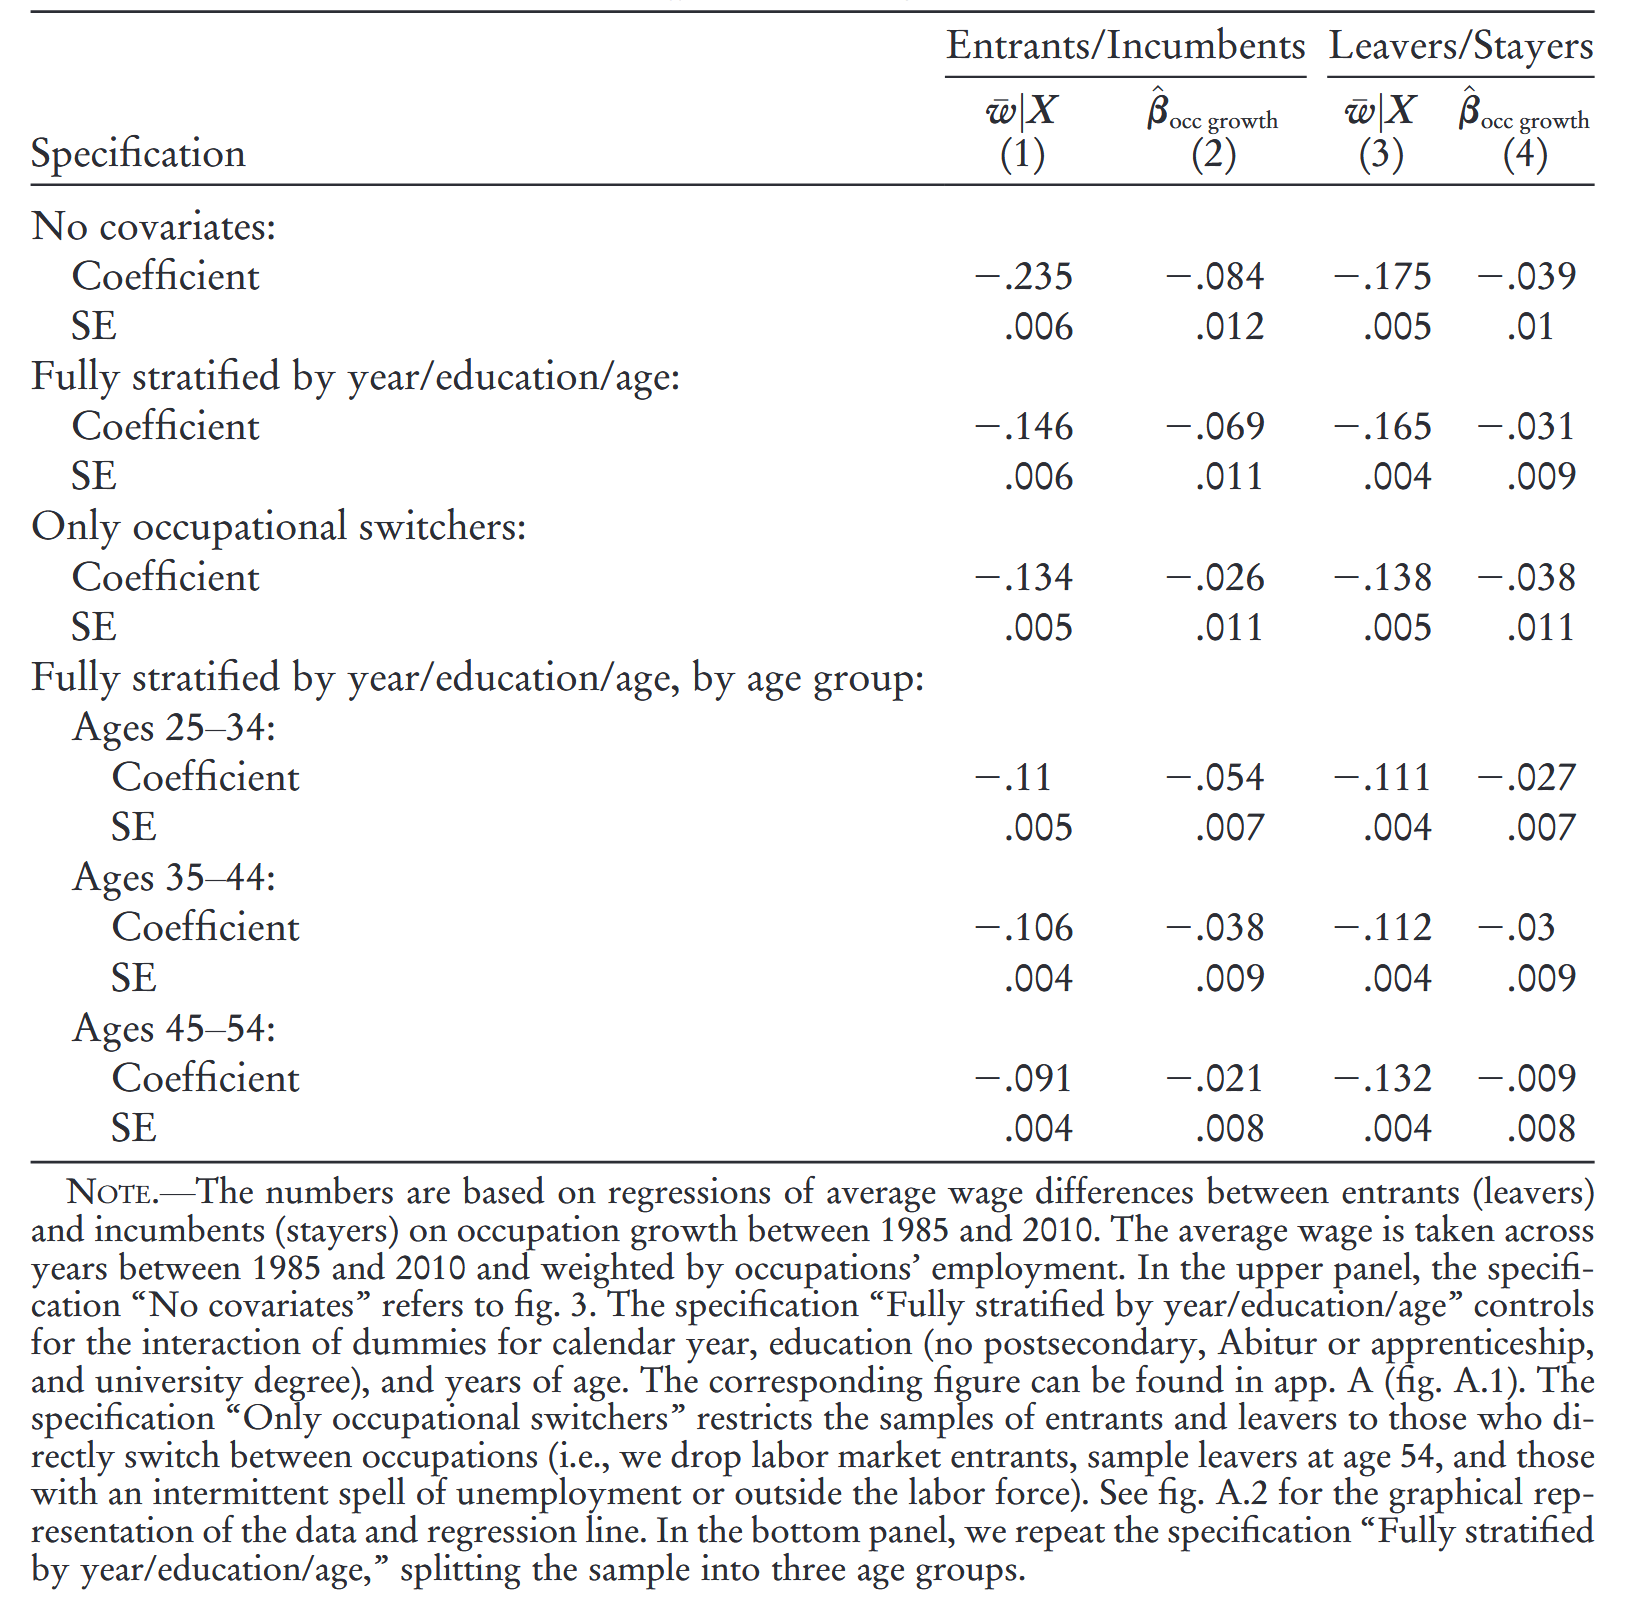
\includegraphics{bohmOccupationGrowthSkill2024_tab1.png}}
        \label{bohmOccupationGrowthSkill2024_tab1}
    \end{center}
\end{figure}

Observables account for $38\%$ of the gap between entrants and incumbents; they explain much less of the differences between leavers and stayers. The bottom panel shows that coefficients drop by another $30\%$ on average when splitting the sample into 10-year age groups, thereby making the pools of marginal and incumbent workers more homogenous in that dimension. Qualitatively, results are the same. \highlightP{These patterns underscore that the wage gaps are related to skill selection in education and age. At the same time, the majority of gaps remain unexplained by standard Mincer variables.} The third row of \ref{bohmOccupationGrowthSkill2024_tab1} investigates the extent to which the gaps persist even among direct occupational switchers (i.e., excluding labor market entrants, sample leavers at age 54, and moves to and from nonemployment). Relative to differences in unconditional wages for the entire sample in the first row, the wage gaps decline by $43\%$ and $21\%$, respectively. This is natural, as this sample removes the large skill differences due to entrants/leavers moving between nonemployment states or young workers entering the labor market. The average wage gap remains substantial. This shows that direct occupation switchers will measurably contribute to skill selection below, and it suggests once more that skills are occupation specific.

In all specifications contained in \ref{bohmOccupationGrowthSkill2024_tab1}, the slopes of wage gaps with respect to occupation growth are negative. This underscores that when occupations grow, the composition of workers changes so that average skills become increasingly scarce at all margins -- in terms of observables and unobservables and among workers hired directly from other occupations. The last two columns of table 1 are related to \citet{groesUShapesOccupationalMobility2015} analysis of the Danish labor market. Also using a sample of stayers and leavers, they find that both low and high earners in an occupation are most likely to switch. In our German data, low earners in an occupation have a much higher probability of leaving, dominating the average differences between leavers and stayers (see app. A, sec. A.3).

The prominent models in the literature on occupational changes have difficulty matching the facts in figure \ref{bohmOccupationGrowthSkill2024_fig3} and \ref{bohmOccupationGrowthSkill2024_tab1}, as they feature one-dimensional skills. A single dimension leads to a hierarchical ranking of occupations by skill and ensures tractability in general equilibrium. It also implies that upward switchers leave the lower-ranked occupation from above and that downward switchers enter lower-ranked occupations from above. This is hard to square with the finding that even entrants and leavers in low-wage occupations generally earn less than incumbents and stayers, respectively. In principle, the model in \citet{hsiehAllocationTalentUS2019} could deliver the empirical facts from figure \ref{bohmOccupationGrowthSkill2024_fig2}, figure \ref{bohmOccupationGrowthSkill2024_fig3}, and \ref{bohmOccupationGrowthSkill2024_tab1}. To make quantitative predictions, it requires time-constant skills and parametric assumptions about individual skills in all sectors.  

The remainder of this paper develops and estimates an empirical model with multidimensional skills that flexibly change over the career. For estimation we only require data on age, occupations chosen, and the corresponding wages. We will use this model to explain and quantify the implications of the new stylized facts shown in this section.

\section{Estimating Skill Prices with Longitudinal Data}

There are $K$ distinct occupations. At any time $t$ a worker $i$ would earn potential wage $W_{i, t, k}$ in occupation $k$. This potential wage is the product of the worker's occupation-specific skill $S_{i, t, k}$ and the occupation-specific price for a unit of skilled labor $\Pi_{t, k}$. We use lowercase letters to denote logs. As in Roy (1951), we assume that workers maximize their incomes by choosing the occupation in which they earn the highest wage:
\begin{equation}
    \label{bohmOccupationGrowthSkill2024_eq1}
    w_{it} = \max\bc{w_{i,t,1}, \ldots, w_{i,t,K}} = w_{i, t, k\of{i,t}} = \pi_{t, k\of{i,t}} + s_{i, t, k\of{i,t}}.
\end{equation}
The occupation subscipt's argument $\bp{i,t}$ indicates that $k$ is $i$'s choice at time $t$.

Our goal is to estimate the evolution of skill prices $\pi_{t,k}$ over time. Based on equation (\ref{bohmOccupationGrowthSkill2024_eq1}), we first employ an approximation that allows us to disentangle prices from skills based on observed data. In the empirical formulation, prices evolve at the aggregate level. Skills will grow and be subject to idiosyncratic shocks over an individual's career; we describe how we deal with the challenges that arise from this in a second step.

The Roy model is hard to estimate in its general form (\ref{bohmOccupationGrowthSkill2024_eq1}) and requires strong restrictions. \citet{bohmPricePolarizationEstimating2020} derives a computationally simple approximation, which he uses in repeated cross-section data under the assumption that observable and time-invariant proxies for each $s_{i,t,k}$ are available. We adapt \citeauthor{bohmPricePolarizationEstimating2020}'s result to a panel data setting.

For a worker who switches occupations (i.e., $k\of{i,t-1} \neq k\of{i,t}$), note from equation (\ref{bohmOccupationGrowthSkill2024_eq1}) that 
\begin{equation}
    \notag 
    w_{i, t-1, k\of{i,t}} - w_{i, t-1, k\of{i,t-1}} \leq 0 \quad w_{i,t,k\of{i,t}} - w_{i, t, k\of{i, t-1}} > 0.
\end{equation}
We also assume the following:
\begin{assumption}
For workers who switch occupations, one can approximate the wage at indifference, where 
$$w_{i, \tau, k\of{i,t}} = w_{i, \tau, k\of{i,t-1}}, \tau \in [t-1, t),$$
to be in the middle of the wage interval 
$$\bs{\bp{w_{i, t-1, k\of{i,t}} - w_{i, t-1}, k\of{i, t-1}}, \bp{w_{i, t, k\of{i,t}} - w_{i, t, k\of{i, t-1}}}}.$$
That is, we assume the switch point to be halfway between the previous and the current relative wage:
\begin{equation}
    \label{bohmOccupationGrowthSkill2024_eq2}
    \underbrace{w_{i, t-1, k\of{i,t}} - w_{i, t-1, k\of{i, t-1}}}_{\text{relative wage in period $t-1$}} + \underbrace{w_{i, t, k\of{i,t}} - w_{i, t, k\of{i, t-1}}}_{\text{relative wage in period $t$}} = 0.
\end{equation}
\end{assumption}

For occupation switchers, the Roy model implies negative relative wages in $t-1$ and positive relative wages in $t$. \highlightO{Assumption 1 posits that the absolute values of these relative wages (i.e., the wage rents from the chosen occupation or the wage distance to indifference) are the same in both periods.} From this, we can express realized wage changes as a function of potential wage changes in the occupations worker $i$ chooses in $t-1$ and $t$.

\begin{result}
Under Assumption 1, worker $i$'s observed wage growth between $t-1$ and $t$ can be written in terms of the potential wage growth in the occupations he chooses in those periods:
\begin{equation}
    \label{bohmOccupationGrowthSkill2024_eq3}
    \D w_{i,t} = \frac{1}{2} \bp{\D w_{i, t, k\of{i,t}} + \D w_{i, t, k\of{i, t-1}}},
\end{equation}
where 
$$
\D w_{i, t, k\of{i,t}} \coloneqq w_{i, t, k\of{i, t}} - w_{i, t-1, k\of{i, t}}, \quad \D w_{i, t, k\of{i, t-1}} \coloneqq w_{i, t, k\of{i,t-1}} - w_{i, t-1, k\of{i, t-1}}.
$$
\end{result}

Result 1 is economically attractive as it includes workers' endogenous switches between occupations due to changing potential wages. Naturally, if a worker stays in an occupation during two adjacent periods, his realized wage change is equal to the change in his potential wage in the chosen occupation. If the worker decides to switch occupations and $k\of{i, t-1} \neq k\of{i, t}$, half of his wage gain stems from the wage change he would have experienced had he stayed in his previous occupation ($\D w_{i, t, k\of{i,t-1}}$). The other half is the wage change had he been in the current occupation all along ($\D w_{i, t, k\of{i,t}}$). Importantly, only potential wages in the previous and current occupations matter for $i$'s observed wage change; potential wages in all other occupations are irrelevant. This stems from the fact that the worker has comparative advantage in both of these occupations and that he chooses accordingly.

Using equation (\ref{bohmOccupationGrowthSkill2024_eq1}), we can decompose result 1 into changes of prices and skills:
\begin{equation}
    \label{bohmOccupationGrowthSkill2024_eq4}
    \D w_{i,t} = \frac{1}{2} \bp{\D \pi_{t, k\of{i,t}} + \D s_{i, t, k\of{i,t}}} + \frac{1}{2} \bp{\D \pi_{t, k\of{i, t-1}} + \D s_{i, t, k\of{t-1}}}.
\end{equation}
In the next section, we show how panel data on wages and occupation choices allow us to estimate the evolution of prices and skills imposing minimal yet informative structure on $\D s_{i, t, k}$.

\subsection{Identification of Skill Prices Changes}

The empirical strength of result 1 is that both individuals' realized wage changes $\D w_{i,t}$ and occupation choices $k\of{i, t-1}, k\of{i,t}$ are observed in the SIAB data. This allows linking potential and observed wage changes. However, we need to put more structure on equation (\ref{bohmOccupationGrowthSkill2024_eq4}) in order to separate changes in skill prices from changes in skills. Our framework relies on differences. We thus do not place restrictions on either object's initial levels.

We model the skill accumulation process as learning-by-doing on the job. Its speed is occupation specific and depends on age; working in one occupation $k$ impacts subsequent skills in all other occupations. In particular, we assume the following.

\begin{assumption}
Individuals' occupation-specific changes are time invariant in expectation. For all $k \in \bc{1, \ldots, K}$ and $i \in \bc{1, \ldots, N}$,
\begin{equation}
    \label{bohmOccupationGrowthSkill2024_eq5}
    \E\bs{\D s_{i, t, k} \mid a\of{i, t-1}, k\of{i, t-1}, k} = \G_{a\of{i, t-1}, k\of{i, t-1}, k},
\end{equation}
with $a\of{i, t-1}$ denoting the age group of individual $i$ in period $t-1$. 
\end{assumption}

Assumption 2 restricts reduced-form parameters to be time invariant. It can be interpreted as consiting two restrictions. \highlightP{The first restriction is time invariance of the structural skill accumulation parameters introduced later.} This means that ex ante skill accumulation within $a\of{i, t-1} \times k\of{i, t-1}$ cells for all potential $k$ has not changed over time. This is consistent with the literature studying occupational changes, and more generally with the idea that differences in returns to worker characteristics over time are due to changes in the returns to skills rather than changes in skill endowments.

\highlightP{The second restriction assumes that chaning prices do not affect ex post observed skill accumulation among workers of age $a\of{i, t-1}$ with realized choices $k\of{i, t-1}$ and $k\of{i, t}$.} \highlightR{This is at odds with the idea of self-selection in the Roy model. The latter would imply, for example, that workers who stay in an occupation during a period of declining prices will be positively selected on skill changes compared with staying workers in periods with constant prices.} Therefore, on the one hand, our approach makes progress compared with the literature by incorporating workers' endogenous choices based on changing potential wages. On the other hand, it retains the limitation that skill accumulation parameters are not adjusted for changing self-selection over time. 

To examine the plausibility of assumption 2 empirically, figure \ref{bohmOccupationGrowthSkill2024_fig4} plots the year-to-year wage growth of 25-34-year-olds and 35-44-year-olds (B) minus average wage growth of 45-54-year-olds. We subtract the overall mean everywhere. Under assumption 2, the ratio of wage growth across different demographic cells should remain constant over time; the eight lines should thus be flat at zero. In figure \ref{bohmOccupationGrowthSkill2024_fig4}B, all lines come close to it. Figure \ref{bohmOccupationGrowthSkill2024_fig4}A is somewhat noisier, but there are no systematic trends. These results suggest that within occupations, relative wage growth of different age groups has not substantively changed over time. 

\setcounter{figure}{3}
\renewcommand{\thefigure}{\arabic{figure}}
\begin{figure}[H]
    \noindent\caption{Individual wage growth relative to 45-54-year-olds}
    \begin{center}
        \resizebox{1\textwidth}{!}{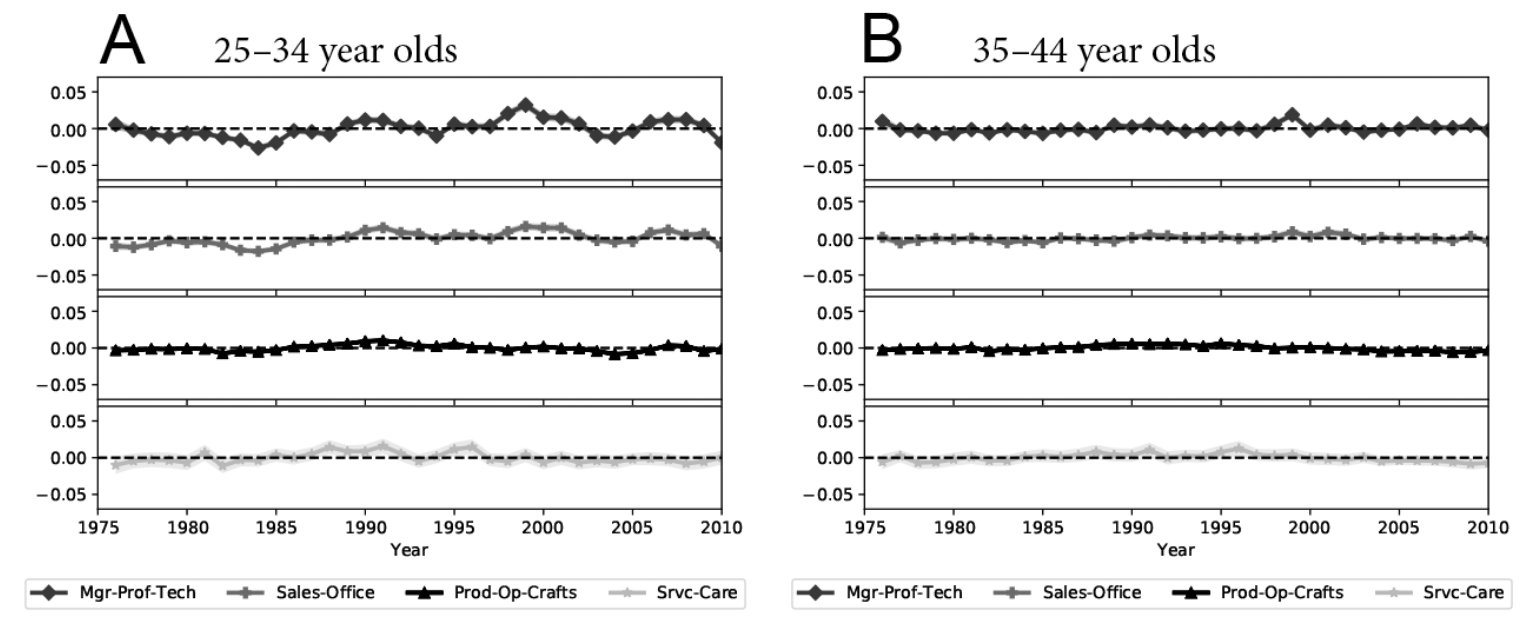
\includegraphics{bohmOccupationGrowthSkill2024_fig4.png}}
        \label{bohmOccupationGrowthSkill2024_fig4}
    \end{center}
    {\footnotesize The lines show average individual wage growth from $t-1$ to $t$ by year of 25-34-year-olds (A) and 35-44-year-olds (B) minus average wage growth of 45-54-year-olds. Results are centered at zero to show trends over time. The shaded areas around the four lines are 95\% confidence intervals. The four groups are based on an aggregation of detailed occupations in the SIAB scientific use file, as described in table A.1. A color version of this figure is available online.}
\end{figure}

Assumption 2 identifies changes in skill prices from the difference between wage changes and expected skill changes up to a constant. We thus need one further normalization, which we apply to skill price growth during part of our sample. 

\begin{assumption}
Skill prices are constant during a base period, that is, 
\begin{equation}
    \notag 
    \D \pi_{t, k} = 0, \quad \forall k \in \bc{1, \ldots, K}, t \in \bc{1, \ldots, T_{\text{base}}}.
\end{equation}
\end{assumption}

\highlightP{Under assumption 3, $\G$ is identified from the base period due to its time-invariant nature.} Accordingly, the estimates of $\D \pi_{t,k}$ can be interpreted as actual changes of skill prices for $t > T_{\text{base}}$. Distinguishing between price and skill growth is a general challenge of estimation based on panel data; it is often done rather implicitly. Using the whole decade 1975-84 as the base period, we will abstract from short-term fluctuations. This period covers the entire business cycle.

Another identification strategy is to assume that seasoned workers' average skill growth is zero (``flat spot identification''). Under this assumption, occupation-specific wage growth over the decades is identical to price growth for these ages. Wage growth still incorporates endogenous choices, as in result 1. We will explore this as a robustness check, finding results similar to our specification.

\subsection{Estimation and Interpretation of Skill Accumulation Parameters}

We combine the equation for wage growth (\ref{bohmOccupationGrowthSkill2024_eq4}) and skill accumulation equation (\ref{bohmOccupationGrowthSkill2024_eq5}) to obtain our baseline estimation equation:
\begin{equation}
    \label{bohmOccupationGrowthSkill2024_eq6}
    \begin{aligned}
        \D w_{i,t} & = \D \pi_{t, k\of{i, t-1}} \cdot \frac{\ind{k\of{i, t-1}}}{2} + \D \pi_{t, k\of{i, t}} \cdot \frac{\ind{k\of{i,t}}}{2} \\
        & + \G_{a\of{i,t-1}, k\of{i, t-1}, k\of{i,t-1}} \cdot \frac{\ind{a\of{i, t-1}} \cdot \ind{k\of{i, t-1}}}{2} + \\
        & + \G_{a\of{i, t-1}, k\of{i, t-1}, k\of{i, t}} \cdot \frac{\ind{a\of{i,t-1}} \cdot \ind{k\of{i, t-1}} \cdot \ind{k\of{i,t}}}{2} + \ve_{i, t},
    \end{aligned}
\end{equation}
with $\ind{a\of{i,t}}$ and $\ind{k\of{i,t}}$ denoting indicator variables for $i$'s age group and choice of occupation, respectively. In line with assumption 3, we set $\D \pi_{k,t} = 0 \forall k \in \bc{1, \ldots, K}, t \in \bc{1, \ldots, T_{\text{base}}}$ and estimate equation (\ref{bohmOccupationGrowthSkill2024_eq6}) for the whole period $t \in \bc{1, \ldots, T}$ by OLS.

Regression (\ref{bohmOccupationGrowthSkill2024_eq6}) is perfectly saturated in age groups, previous occupations, and current occupations. The regression error $\ve_{i,t}$ reflects individuals' skill shocks or idiosyncratic deviations that are different from the average worker in the respective cell spanned by these dummies. That is, we can write $\ve_{i,t} = (1/2) \bp{u_{i, t, k\of{i, t-1}} + u_{i, t, k\of{i,t}}}$, where $u_{i, t, k} \coloneqq \D s_{i, t, k} - \G_{a\of{i, t-1}, k\of{i, t-1}, k}$. By assumption 2 we have $\E\bs{u_{i, t, k} \mid a\of{i, t-1}, k\of{i, t-1}, k} = 0$, and the error term in equation (\ref{bohmOccupationGrowthSkill2024_eq6}) is uncorrelated with the regressors.

\begin{result}
Under assumptions 1-3, OLS estimation of equation (\ref{bohmOccupationGrowthSkill2024_eq6}) consistently identifies changes \\
$\bc{\D \pi_{t,k} \mid t > T_{\text{base}}}$ and average skill changes $\bc{\G_{a\of{i, t-1}, k\of{i, t-1}, k}}$. Without assumption 3, OLS identifies these parameters up to the normalization of the base period.
\end{result}

As discussed with assumption 2, average occupation-specific skill changes $\G$ will not coincide with structural skill accumulation parameters in general. Suppose there exists a learning-by-doing production function, such that ex ante a worker accumulates skills according to 
\begin{equation}
    \notag 
    \G^*_{a\of{i, t-1}, k\of{i, t-1}, k} = \E\bs{\D s_{i, t, k} \mid a\of{i, t-1}, k\of{i, t-1}} + u^*_{i, t, k}.
\end{equation}
What we identify in regression (\ref{bohmOccupationGrowthSkill2024_eq6}) is ex post accumulation in the sense that 
\begin{equation}
    \label{bohmOccupationGrowthSkill2024_eq7}
    \G_{a\of{i, t-1}, k\of{i, t-1}, k\of{i,t}} = \G^*_{a\of{i, t-1}, k\of{i, t-1}, k\of{i,t}} + \E\bs{u^*_{i, t, k} \mid a\of{i, t-1}, k\of{i, t-1}, k\of{i,t}}
\end{equation}
is conditional on the current choice $k\of{i,t}$ and $u_{i,t,k} = u^*_{i, t, k} - \E\bs{u^*_{i, t, k} \mid a\of{i, t-1}, k\of{i, t-1}, k\of{i,t}}$ is the deviation of the structural shock from its ex post mean. By the nature of the data, $\G_{a\of{i,t-1}, k\of{i,t-1}, k}$ with $k\of{i, t-1} \neq k$ will be identified from switchers. For those, often 
\begin{equation}
    \notag 
    \E\bs{u^*_{i, t, k} \mid a\of{i, t-1}, k\of{i, t-1}, k\of{i,t}} > \E\bs{u_{i,t,k}^* \mid a\of{i, t-1}, k\of{i, t-1}}.
\end{equation}
That is, the off-diagonal accumulation parameters tend to be upward biased because of a classic self-selection problem. We thus cannot interpret them as what is learned for $k\of{i,t}$ while working in $k\of{i, t-1}$ in the entire population. More subtly, stayers' $\G_{a\of{i,t-1}, k\of{i,t-1}, k\of{i,t}}$ with $k\of{i,t-1} = k\of{i,t}$ will tend to be overestimated relative to $\G^*$, too. By self-selection, stayers are likely to have experienced more positive shocks compared with leavers.

Nevertheless, regression (\ref{bohmOccupationGrowthSkill2024_eq6}) succeeds in estimating the skill price changes as long as assumption 2 holds. The price changes are well identified using our method for plausible parameter ranges. It becomes clear, however, that the estimated $\G$ matrix needs too be interpreted in the above ex post sense. For our decomposition purposes and analysis of skills in occupations, this will be sufficient. The caveats are that we can make statements neither about workers' skill (changes) in occupations that they do not choose nor about the population distribution of the $K$-dimensional skill vector. 

\section{Skill Prices and Skill Selection}

This section first presents the estimation results. These include the evolution of skill prices, the accumulation of skills over the career, and the relationship of prices and occupations' average skills with employment growth. We then dig deeper into the nature of the implied selection effects, showing that the skill differences between marginal workers and those who remain in their occupations drive the strongly negative association of employment growth with average skill changes in an occupation. We further decompose these in section 4.3 before reporting on various robustness exercises in the final part. One of those is an alternative way to think about unemployment and spells outside the labor force, which are not fully obvious in our setup (in the main estimation, we treat such spells as missing data).

\subsection{Estimated Skill Price Changes and Average Skill Accumulation}

Figure \ref{bohmOccupationGrowthSkill2024_fig5}A depicts the evolution of skill prices, normalizing them to zero in 1985 and cumulating the yearly changes until 2010. In the broad occupation groups, skill prices increased strongly among Mgr-Prof-Tech occupations, increased modestly among Sales-Office and Srvc-Care, and decreased among Prod-Op-Crafts. The thin lines in the background show that these broad estimates mask substantial heterogeneity among the 120 detailed occupations. We will explore this in greater detail below.

\begin{figure}[H]
    \noindent\caption{Estimated skill prices and stayers' average skill accumulation}
    \begin{center}
        \resizebox{1\textwidth}{!}{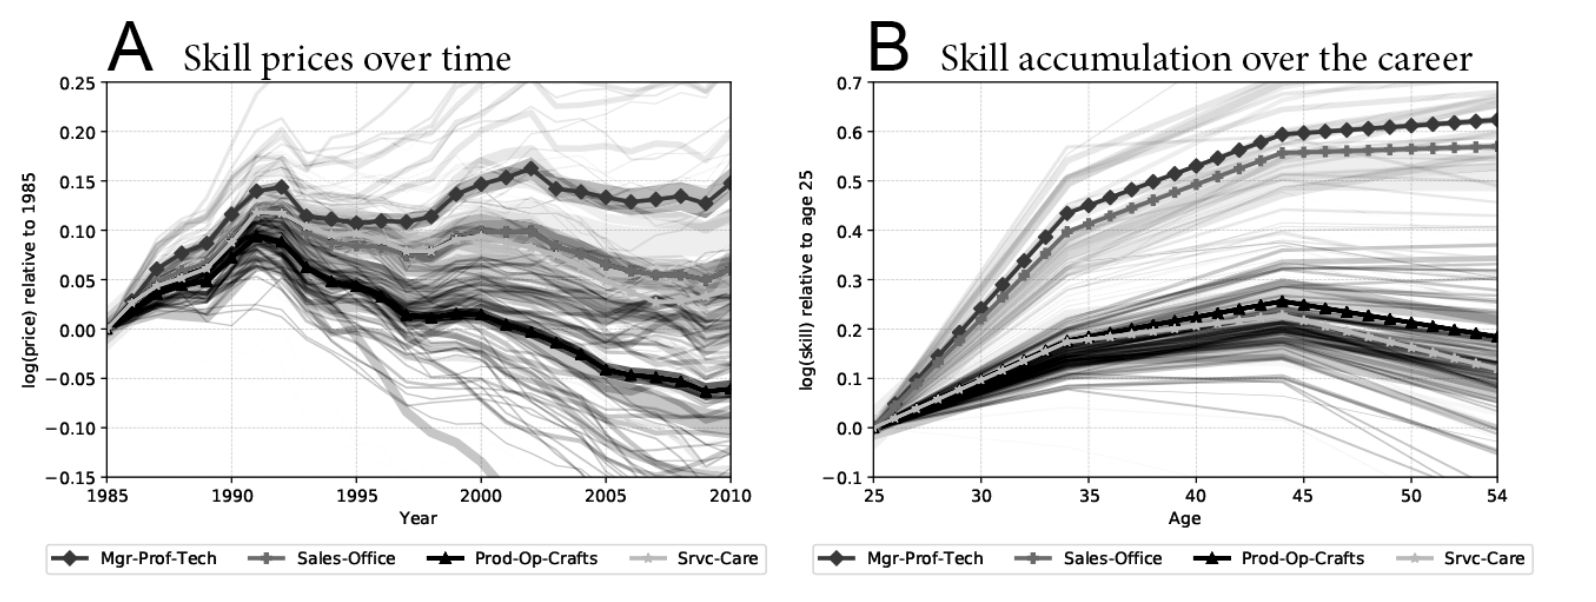
\includegraphics{bohmOccupationGrowthSkill2024_fig5.png}}
        \label{bohmOccupationGrowthSkill2024_fig5}
    \end{center}
    {\footnotesize The graphs show estimated skill price changes over time and occupation stayers' skill accumulation over the life cycle. OLS estimates are as described by equation (\ref{bohmOccupationGrowthSkill2024_eq6}). Shaded lines in the background represent the 120 detailed occupations in the SIAB scientific use file. The four groups show an aggregation of these detailed occupations, as described in table A.1. The thickness of a shaded background line corresponds to the number of employed workers in an occupation averaged across years 1985 until 2010. The shaded areas around the four lines are 95\% confidence intervals. A color version of this figure is available online.}
\end{figure}

Several distinct periods are noticeable. All prices increased in the favorable economic conditions between 1985 and 1991, although this was already less pronounced for the Prod-Op-Crafts occupations. These have experienced a continuous decline thereafter to the point that prices in 2010 were more than $5\%$ below their initial value in 1985. For the other occupations, there was a drop during the 1992-93 recession as well; prices then stayed constant until they rebounded before the turn of the century. This rebound was most pronounced for Mgr-Prof-Tech occupations; prices in this group did not change much for the remainder of our sample period. Skill prices fell by about $5$ percentage points for Sales-Office and Srvc-Care occupations between 2000 and 2010. These broad patterns are consistent with the job polarization of figure \ref{bohmOccupationGrowthSkill2024_fig1}B.

Figure \ref{bohmOccupationGrowthSkill2024_fig5}B graphs the estimates for the diagonal elements of $\bds{\G}$, that is, the average skill accumulation for stayers. Skill growth in the early years of the career is steep. Absent changes in skill prices, it implies a $20\%$ growth in wages between age 25 and age 34 for Prod-Op-Crafts or Srvc-Care occupations and $50\%$ or more for the other two. It slows down midcareer and flattens out or turns negative toward the end of prime age. This reflects the wellestablished concavity of life cycle wage profiles. Skill growth differs substantially by occupation. It is initially fast in highearning Mgr-Prof-Tech and Sales-Office occupation groups and never completely ceases. Growth is flatter and eventually peters out or turns negative in the Prod-Op-Crafts and Srvc-Care groups (i.e., occupations that often require physical labor). Again, the broad groups mask substantial heterogeneity across the detailed occupations. At the same time, it is the case that the MgrProf-Tech and Sales-Office occupations on the one hand and the Prod-OpCrafts and Srvc-Care occupations on the other hand are almost separate; there are hardly any to be found in the other block. This shows that life cycle wage profiles are decidedly different across occupations, and accounting for this is critical in producing reasonable estimates of prices and skills.

We now hone in our key finding of this section, namely, that employment growth and skill price growth go hand in hand. Figure \ref{bohmOccupationGrowthSkill2024_fig2}A has shown that the LHS (i.e., the average wage change of professions over the 1985-2010 period) is unrelated to employment growth at the level of the 120 detailed occupations. Figure \ref{bohmOccupationGrowthSkill2024_fig6} plots its two components on the right-hand side separately.
\begin{equation}
    \label{bohmOccupationGrowthSkill2024_eq8}
    \begin{aligned}
        \E\bs{w_{i, t, k\of{i,t}}} - \E\bs{w_{i, t-1, k\of{i, t-1}}} = & \underbrace{\D \pi_{t, k}}_{\text{price change}} \\
        & + \underbrace{\E\bs{s_{i, t, k\of{i,t}}} - \E\bs{s_{i, t-1, k\of{i, t-1}}}}_{\text{mean skill change}}
    \end{aligned}
\end{equation}

\begin{figure}[H]
    \noindent\caption{Correlation of changes in employment, skill prices, and skills}
    \begin{center}
        \resizebox{1\textwidth}{!}{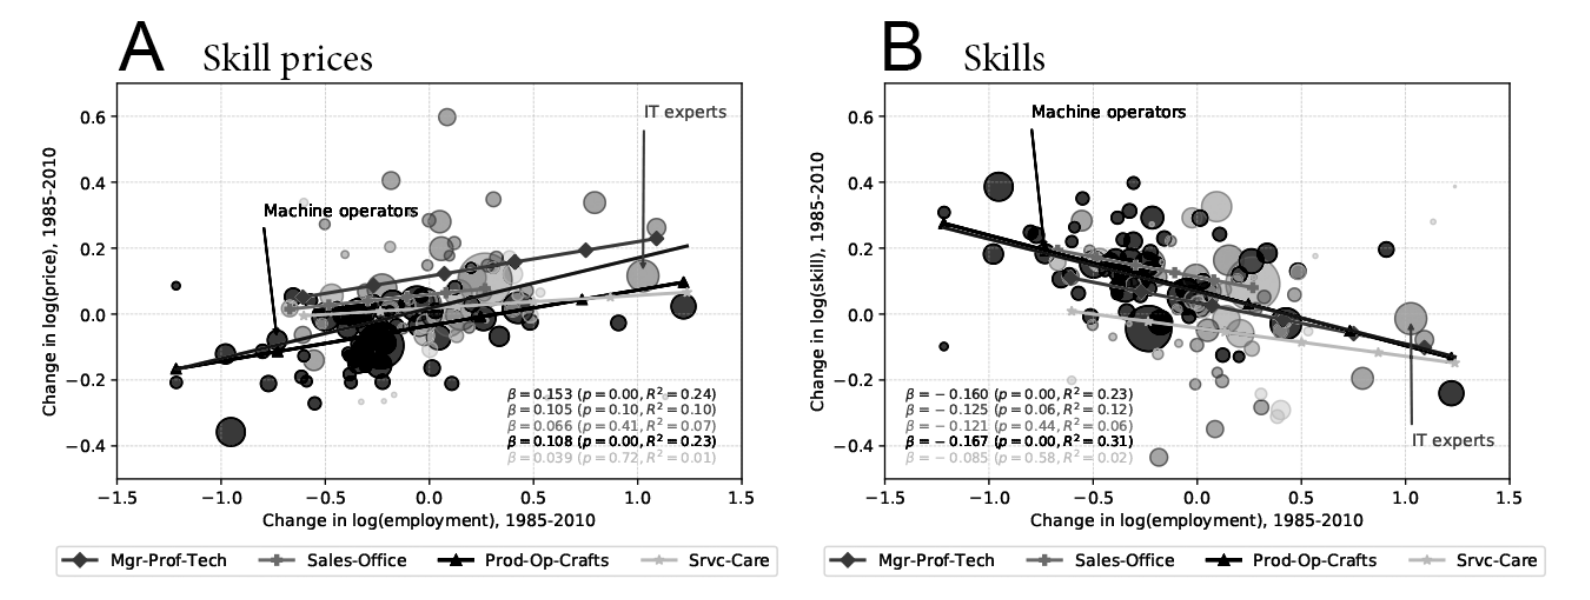
\includegraphics{bohmOccupationGrowthSkill2024_fig6.png}}
        \label{bohmOccupationGrowthSkill2024_fig6}
    \end{center}
    \vspace{-20pt}
    {\footnotesize Notes. The vertical axis in A shows the change in skill prices between 1985 and 2010, estimated as detailed in section 3.2. The vertical axis in B depicts the change in skills between 1985 and 2010, estimated as the residual between price and wage changes as shown in equation (\ref{bohmOccupationGrowthSkill2024_eq8}). The horizontal axis in both panels shows the change in the log number of employed workers within an occupation between 1985 and 2010. One bubble represents one of the 120 detailed occupations in the SIAB scientific use file. The four groups show an aggregation of these detailed occupations, as described in table A.1. Bubble size corresponds to the number of employed workers in an occupation averaged across years 1985 until 2010. Regression lines across all occupations (black) and within the four broad groups (symbols) are weighted by the number of employed workers. A color version of this figure is available online.}
\end{figure}

Figure \ref{bohmOccupationGrowthSkill2024_fig6}A shows that detailed occupations' log employment changes are positively related to cumulative skill price changes over the same period. The black regression line summarizes this strong relationship for the 120 occupations, which is in marked contrast to the zero correlation for wages in figure \ref{bohmOccupationGrowthSkill2024_fig2}A. The relationship holds within occupation groups, showing that the result is more general than a particular demand shifter that predominantly impacts broad occupations. Figure \ref{bohmOccupationGrowthSkill2024_fig6}A indicates that shifts in demand were the dominant driver of occupational employment changes. Pure shifts in supply would have induced a negative correlation of employment with prices, all else equal. At the same time, there exists heterogeneity of occupations' employment and price growth around the regression line(s). This may, among other things, be due to contemporaneous shifts in supply but also due to variation in the elasticity of skill supply (inelastic occupations would have small employment and large price growth).

Figure \ref{bohmOccupationGrowthSkill2024_fig6}B shows that implied skill changes are the flip side of the skill price estimates. The regression line indicates that skills of the occupations with the fastest growth declined by $35$ log points on average compared with those that shrank the most. These are large effects; we devote the next subsections to examining their components and plausibility.

\subsection{Defining and Estimating Employment Growth Selection}

We have documented in section 2.2 that entering (leaving) workers' skills on average appear decidedly below those of incumbents (stayers) and that faster-growing occupations draw even less skilled entrants (leavers). Given that growing sectors by definition experience net entry, this could substantially drag down growing occupations' average wages despite rising demand and increasing skill prices. Here we formalize and quantify this effect in the context of our model, showing that it indeed drives the systematic part of the relationship between employment growth and skills.

The change in average skills of an occupation in equation (\ref{bohmOccupationGrowthSkill2024_eq8}) is determined by three mutually exclusive groups of workers: those who leave the occupation after period $t-1$, those who stay on after period $t-1$ and are thus incumbent in period $t$, and those who enter in period $t$. Denoting the share of leavers after $t-1$ by $p_{t-1, k}^{lvr}$ and the share of period $t$ entrants by $p_{t,k}^{ent}$, we can decompose the change of skills in occupation $k$ into three terms:
\begin{equation}
    \label{bohmOccupationGrowthSkill2024_eq9}
    \begin{aligned}
        \underbrace{\E\bs{s_{i, t, k\of{i,t}}} - \E\bs{s_{i, t-1, k\of{i, t-1}}}}_{\text{mean skill change}} = & \bp{1 - \frac{p_{t-1,k}^{lvr} + p_{t,k}^{ent}}{2}} \cdot \E\bs{\D s_{i, t, k}^{incumb}} \\
        & + \frac{p_{t-1, k}^{lvr} + p_{t, k}^{ent}}{2} \cdot \bp{\E\bs{s_{i, t, k}^{ent}} - \E\bs{s_{i, t-1, k}^{lve}}} \\
        & + \frac{p_{t,k}^{ent} - p_{t-1, k}^{lvr}}{2} \bp{\E\bs{s_{i,t,k}^{ent}} - \E\bs{s_{i,t,k}^{incumb}} + \E\bs{s_{i, t-1, k}^{lvr}} - \E\bs{s_{i, t-1, k}^{sty}}}.
    \end{aligned}
\end{equation}
See section B.4 of appendix B for the steps of the derivation. Summing the year-to-year changes in equation (\ref{bohmOccupationGrowthSkill2024_eq9}) over the period 1985-2010 gives the components of skill changes we analyze in the following.

The first term of equation (\ref{bohmOccupationGrowthSkill2024_eq9}) reflects just this, that is, the skill accumulation of workers who remain in the occupation. Its impact on occupational skill changes is high if turnover is small and skill accumulation of staying workers is high. Figure \ref{bohmOccupationGrowthSkill2024_fig7}A shows that this term is positive for the vast majority of occupations and larger among higher-accumulation occupations.

\begin{figure}[H]
    \noindent\caption{Employment growth versus the components of skill changes}
    \begin{center}
        \resizebox{1\textwidth}{!}{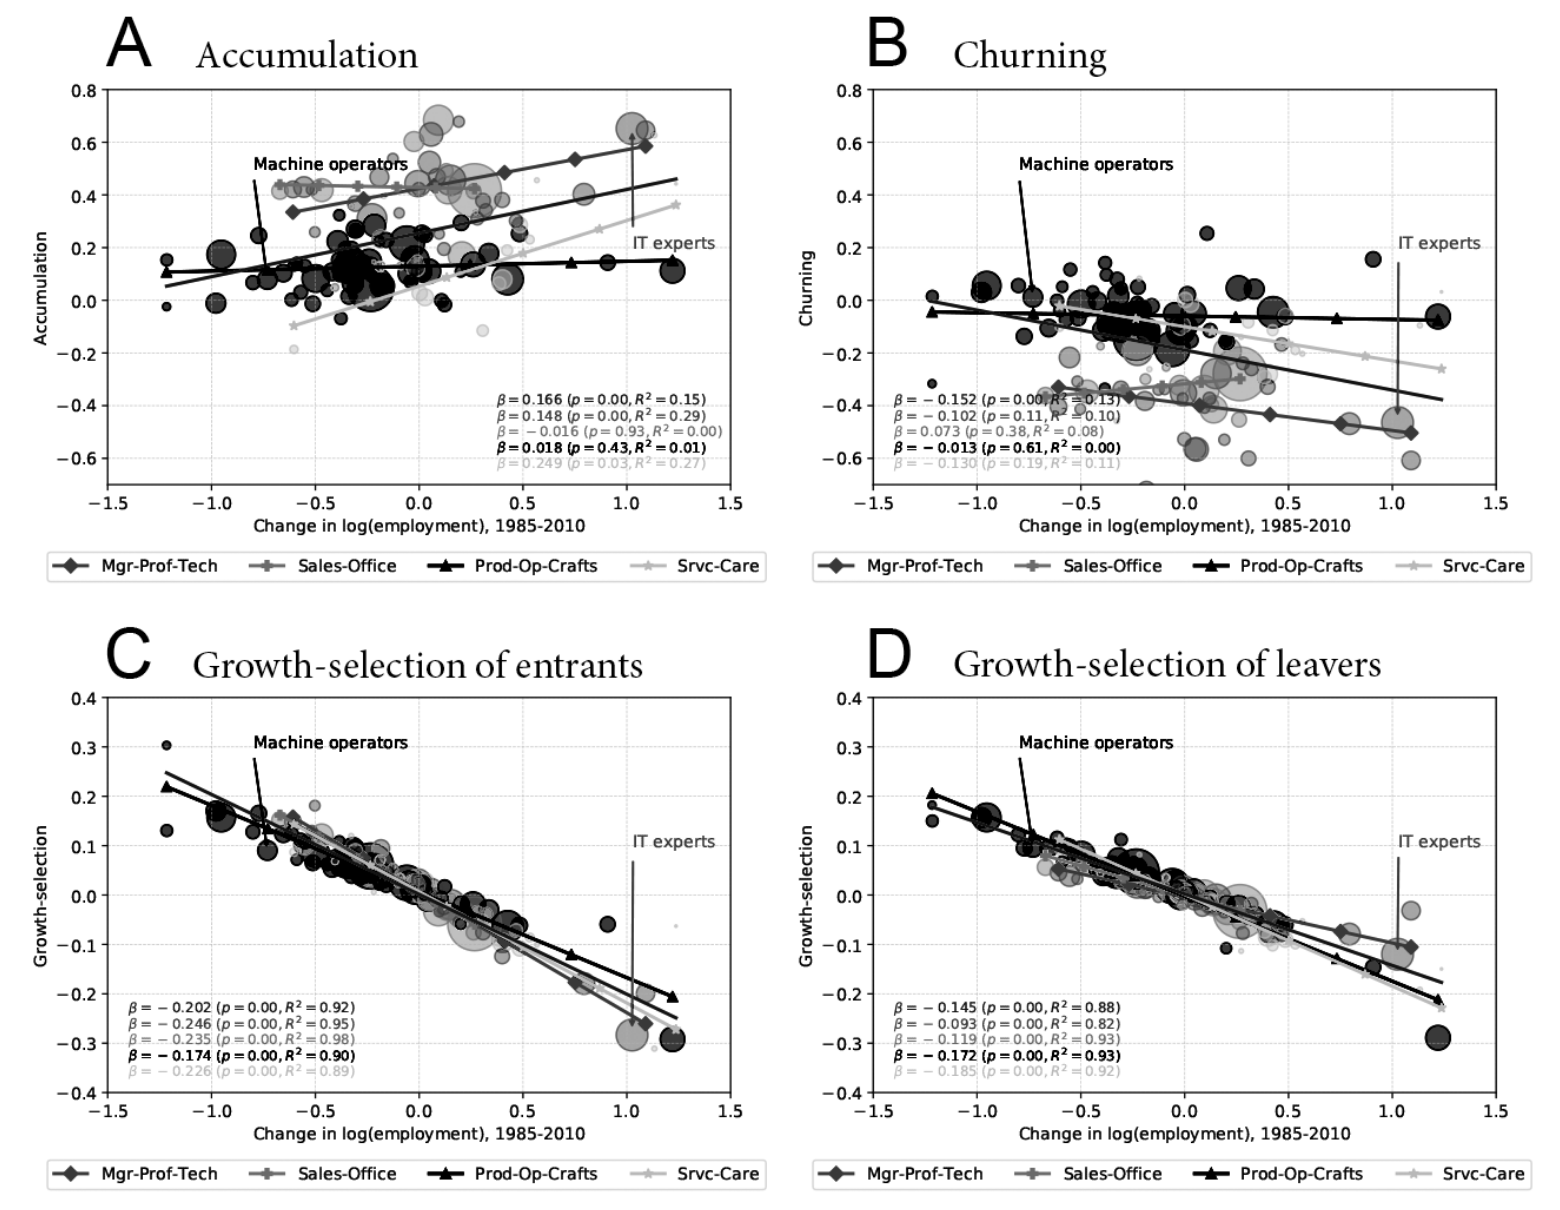
\includegraphics{bohmOccupationGrowthSkill2024_fig7.png}}
        \label{bohmOccupationGrowthSkill2024_fig7}
    \end{center}
    \vspace{-20pt}
    {\footnotesize Notes. Results correspond to sample averages following equation (\ref{bohmOccupationGrowthSkill2024_eq9}). The horizontal axis in both panels shows the change in the log number of employed workers within an occupation between 1985 and 2010. One bubble represents one of the 120 detailed occupations in the SIAB scientific use file. The four groups show an aggregation of these detailed occupations, as described in table A.1. Bubble size corresponds to the number of employed workers in an occupation averaged across years 1985 until 2010. Regression lines across all occupations (black) and within the four broad groups (symbols) are weighted by the number of employed workers. A color version of this figure is available online.}
\end{figure}

The second term of equation (\ref{bohmOccupationGrowthSkill2024_eq9}) is churning, which is composed of average turnover multiplied with the skill differences between period $t$ entrants and $t-1$ leavers. Churning tends to impact aggregate skills negatively, since leavers will have accumulated more skills than entrants. It becomes more negative for high-turnover occupations and for occupations with high levels of skill accumulation. Hence, the accumulation and churning effects will often act in opposite directions. Figure \ref{bohmOccupationGrowthSkill2024_fig7}B shows this to be the case.

Occupation growth does not have a first-order effect on the total of accumulation and churning. By inducing variation in turnover ($p_{t-1, k}^{lvr} + p_{t, k}^{ent}$), occupation growth pushes terms 1 and 2 in opposite directions. It is thus no surprise that the slopes in figure \ref{bohmOccupationGrowthSkill2024_fig7}A and \ref{bohmOccupationGrowthSkill2024_fig7}B have opposite signs. Indeed, we fail to find a systematic relation between their sum and occupation growth (see fig. C.1).

Occupation growth directly enters the third term of equation (\ref{bohmOccupationGrowthSkill2024_eq9}), which we call the ``\highlightB{growth selection effect}''. It is the product of net entry and the skill difference between marginal and inframarginal workers. Because that difference is negative for both entrants and leavers everywhere (see figure \ref{bohmOccupationGrowthSkill2024_fig3}), occupation growth will determine its sign. The growth selection effect is negative for growing occupations, positive for shrinking occupations, and zero when there is no change in size. Growth selection thus formalizes and quantifies the intuition developed in section 2, whereby \highlightPP{the more an occupation grows, the more net entry of less skilled workers it experiences}.

The bottom panels of figure \ref{bohmOccupationGrowthSkill2024_fig7} plot employment growth selection. Both for entrants (fig. \ref{bohmOccupationGrowthSkill2024_fig7}C) and leavers (fig. \ref{bohmOccupationGrowthSkill2024_fig7}D) the relationship between employment growth and growth selection is strongly negative. Both contribute to the declining skills of growing occupations. Growth selection determines the entire negative slope between changes in employment and changes in skills from figure \ref{bohmOccupationGrowthSkill2024_fig6}B (the location of the regression line and most of the variation around it stem from accumulation and churning). Therefore, the systematic part of the large selection effects we found in section 4.1 can be traced back to changes in occupations' sizes multiplied with the skill gaps between marginal and inframarginal workers. An interesting observation is that in the model sketched in section B.1 of appendix B, based on \citet{hsiehAllocationTalentUS2019}, rising skill prices attract workers of exactly offsetting lower quality to an occupation.

\subsection{Contributors to Employment Growth Selection}

Having established its quantitative importance, we now investigate further the nature of the employment growth selection effect. We decompose equation (\ref{bohmOccupationGrowthSkill2024_eq9}) in a way that allows us to gauge the relative contributions of age and of different worker types. That is, is growth selection primarily determined by entry of young workers who simply have not had a chance to accumulate a lot of skills? Or is it that entrants into a growing occupation have lower skills than incumbents had at the same point in their life cycle? Toward the end of this section, we alternatively consider the contributions of different types of switchers (i.e., other occupations, unemployment, etc).



\bibliography{\CiteReference} 

\end{document}